\documentclass[10pt, compress]{beamer}
\usetheme{m}
\usepackage{booktabs}
\usepackage[russian]{babel}
\usepackage[scale=2]{ccicons}
\usepackage{minted}
\usepackage[plain]{algorithm}
\usepackage{algorithmicx}
\usemintedstyle{trac}
\usepackage{varwidth}
\usepackage{xspace}
\usepackage{algpseudocode}
\algnewcommand\algorithmicand{\textbf{and}\xspace}
\algnewcommand\algorithmicor{\textbf{or}\xspace}
\algnewcommand\algorithmicnot{\textbf{not}\xspace}
\algnewcommand\algorithmictrue{\textbf{true}}
\algnewcommand\algorithmicfalse{\textbf{false}}
\algtext*{EndWhile} % Remove "end while" text
\algtext*{EndIf} % Remove "end if" text
\algtext*{EndFor} % Remove "end for" text
\algtext*{EndProcedure} % Remove "end for" text
%---------------------------------------------------------------------------------------

\title{Параллельные алгоритмы поиска кратчайших путей на графах}
\subtitle{}
\date{\today}
\author{Выполнил: Ткаченко Г.C. \\ Руководитель: Корнеев Г.А.}
\institute{Университет ИТМО}

\begin{document}

\maketitle

\section{Проблема и задача}
\begin{frame}[fragile]
  \frametitle{Решаемая проблема}

\begin{itemize}
    \item Низкая производительность отдельных алгоритмов на специфичных графах
    \item Недостаточное разнообразие параллельных алгоритмов для поиска кратчайших путей

  \end{itemize}
\end{frame}

\begin{frame}[fragile]
  \frametitle{Постановка задачи}
\begin{itemize}
    \item Эффективное применение алгоритмов поиска кратчайшего пути на \textbf{многопроцессорных} архитектурах
    \item Разработка алгоритмов для поиска пути от одной вершины до всех (\textbf{one-to-many})
    \item Разработка алгоритмов для поиска пути кратчайшего расстояния между каждой парой вершин (\textbf{many-to-many})
  \end{itemize}
\end{frame}

\section{Задача one-to-many}

\begin{frame}[fragile]
  \frametitle{Обзор решений}
\begin{itemize}
    \item Алгоритм Дейкстры
    \item Алгоритм Беллмана-Форда
    \item Алгоритм Джонсона (Дейкстра с потенциалами)
    \item Алгоритмы A* и D*
  \end{itemize}
\end{frame}

\begin{frame}[fragile]
  \frametitle{Классический Беллман-Форд}
\begin{algorithm}[H]
\begin{algorithmic}[1]
\Procedure{ClassicBellmanFord}{$G,start$}
\State {$dist \gets \left\{ {\infty ... \infty}\right\}$}
\State {$dist[start] \gets 0$}
 
\For{$i = 0$ to $|G.vertices| - 1 $}
	\For{$e \in G.edges $}
		\State $dist[e.to] \gets \min(dist[e.to], dist[e.from] + e.w)$
	\EndFor
\EndFor
\State \textbf{return} $dist$
\EndProcedure
\end{algorithmic}
\end{algorithm}
\end{frame}

\begin{frame}[fragile]
  \frametitle{BFS Беллман-Форд}
\begin{algorithm}[H]
\begin{algorithmic}[1]

\Procedure{BFSBellmanFord}{$G,start$}
\State $dist\gets \left\{ {\infty ... \infty}\right\}$
\State $dist[start] \gets 0$
\State $CurrentVertexSet \gets \left\{ {start}\right\}$
\State $NextVertexSet \gets \emptyset$ 
\While {$CurrentVertexSet.empty()$}
	\State $NextVertexSet.clear()$
	
	\For{$v \in CurrentVertexSet$}
		\For{$e \in G.edgesFrom[v] $} 
			\If {$dist[e.to] > dist[e.from] + e.w$} 
				\State $dist[e.to] \gets dist[e.from] + e.w$
				\State $NextVertexSet.insert(e.to)$								
			\EndIf
		\EndFor
	\EndFor
	
	\State $CurrentVertexSet \gets NextVertexSet$	
\EndWhile
\State \textbf{return} $dist$

\EndProcedure



\end{algorithmic}
\end{algorithm}
\end{frame}

\begin{frame}[fragile]
  \frametitle{Параллельный Беллман-Форд}
  Три подхода
  \begin{itemize}
    \item Параллелизация по ребрам вершины
    \item Параллелизация по всем ребрам
    \item Использование параллельного обхода в ширину
  \end{itemize}
\end{frame}

\begin{frame}[fragile]
  \frametitle{Параллелизация по ребрам вершины}
  {\vspace{-2em}\begin{center}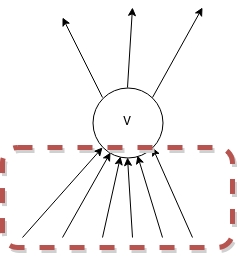
\includegraphics[height=0.75\textheight]{images/bf_par_1.png}\end{center}}
\end{frame}

\begin{frame}[fragile]
  \frametitle{Параллелизация по всем ребрам}
  {\vspace{-2em}\begin{center}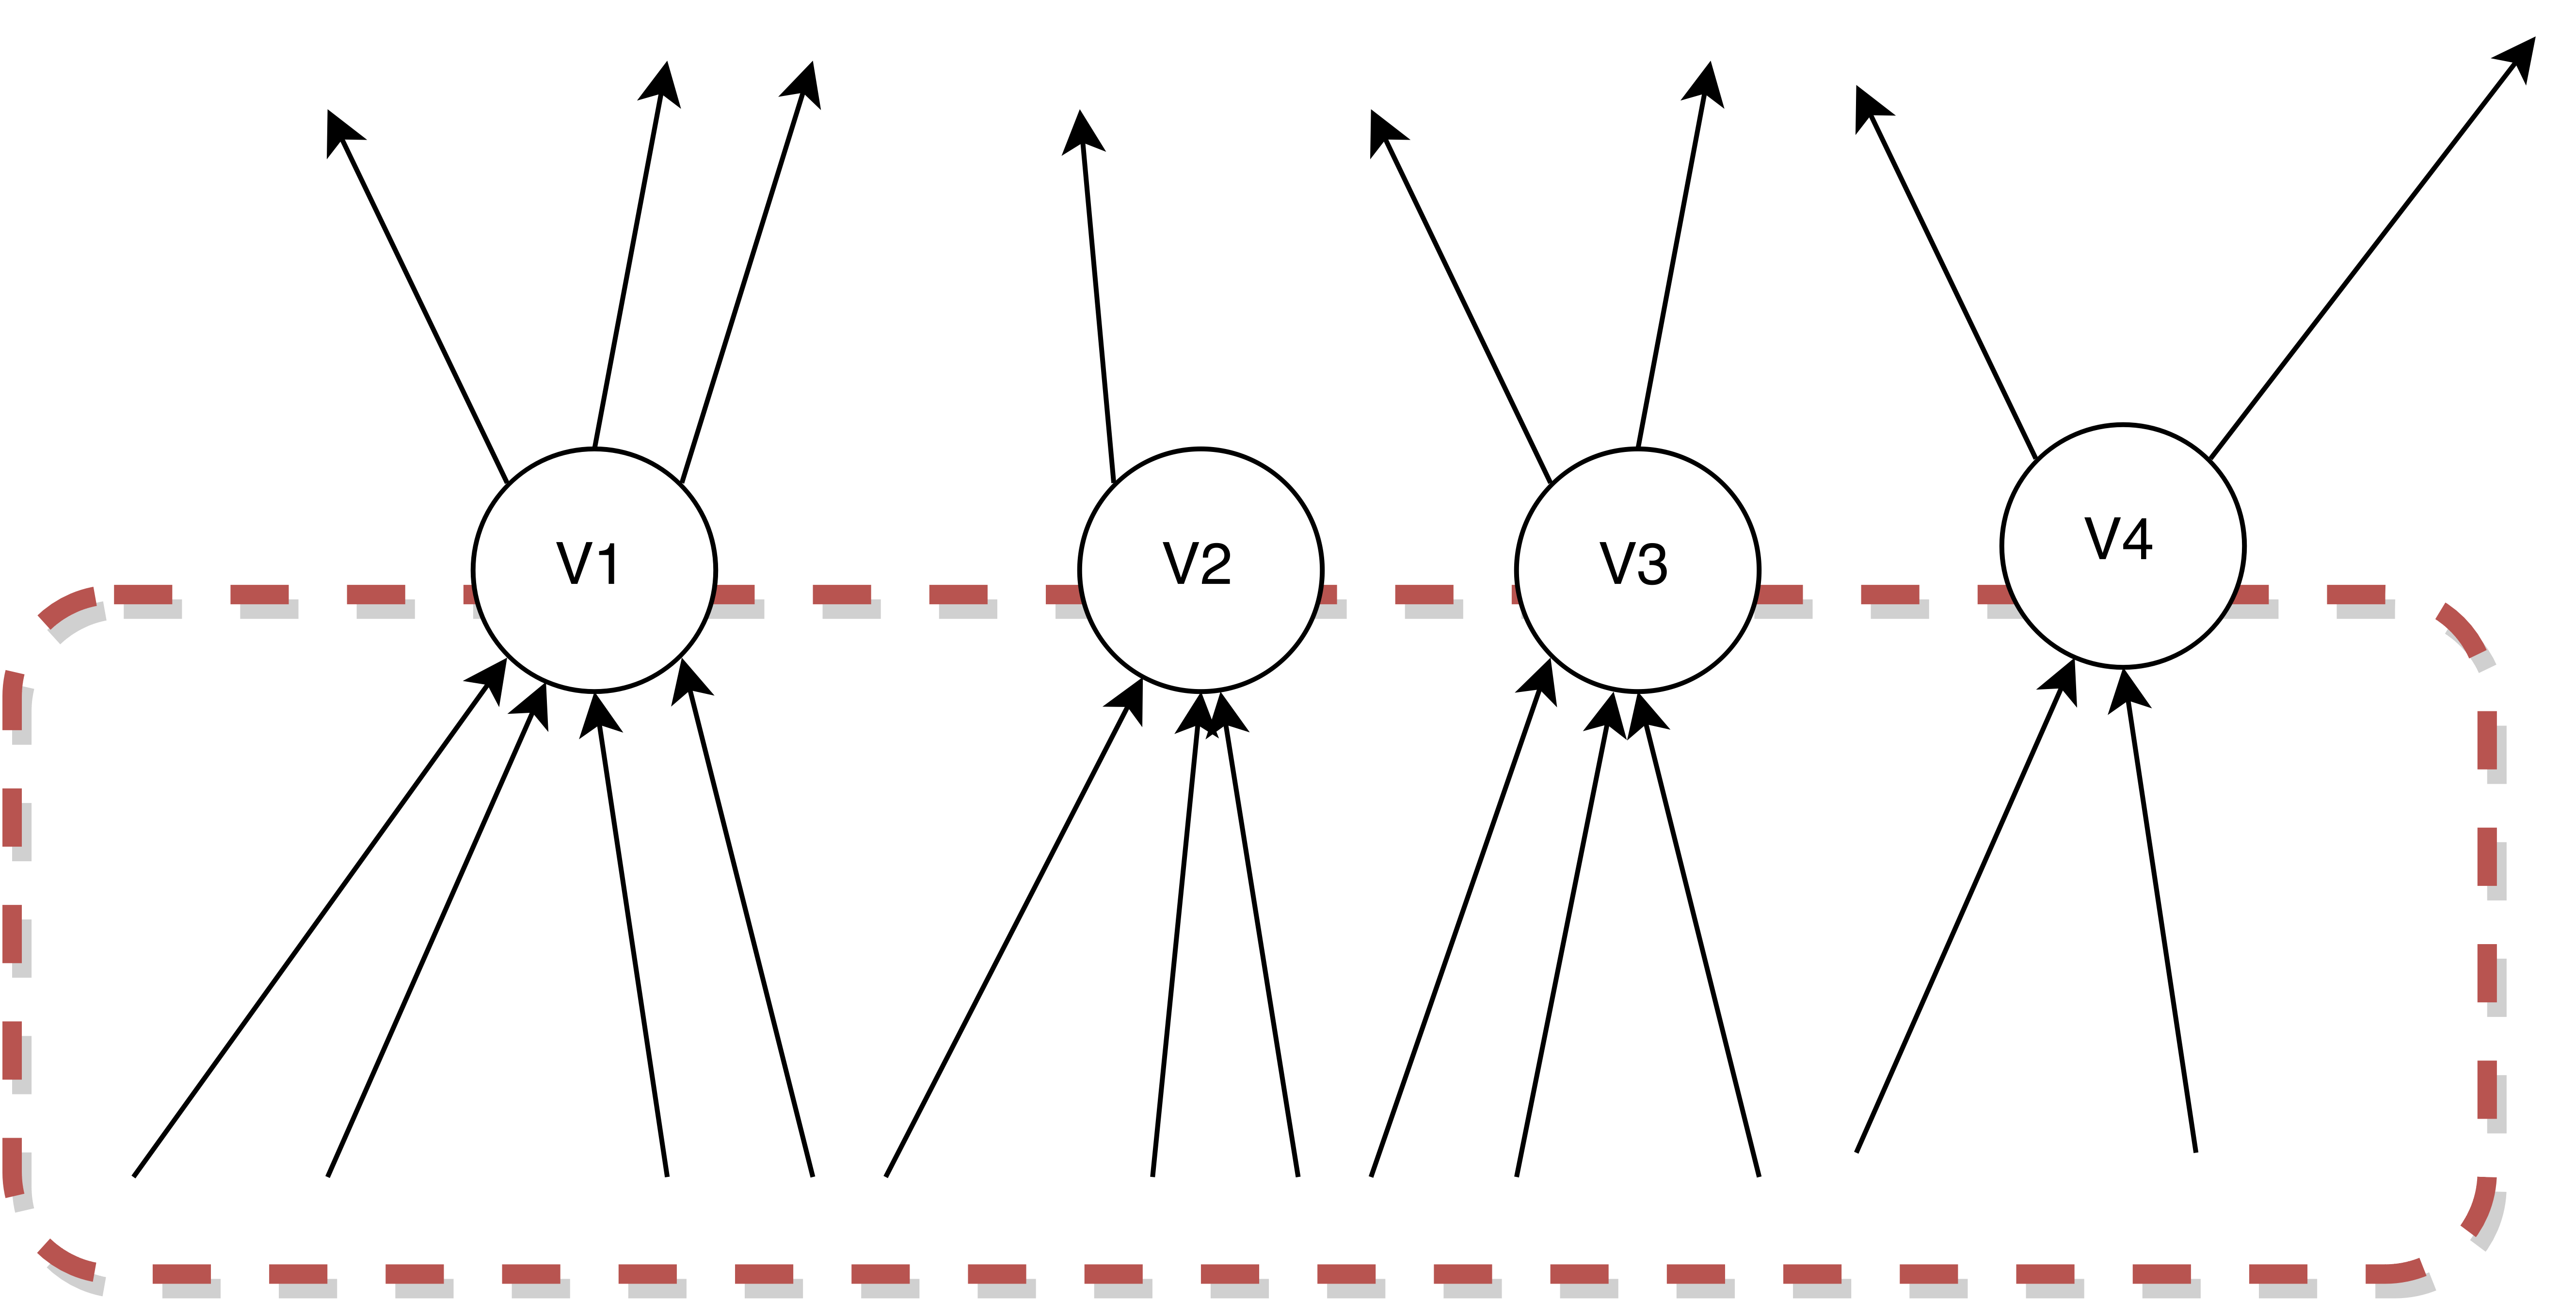
\includegraphics[width=\textwidth]{images/bf_par_2_1.png}\end{center}}
\end{frame}
\begin{frame}[fragile]
  \frametitle{Параллелизация по всем ребрам}
  {\vspace{-2em}\begin{center}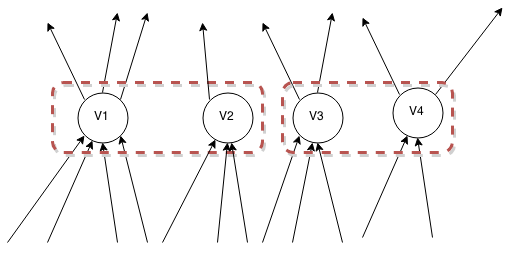
\includegraphics[width=\textwidth]{images/bf_par_2_2.png}\end{center}}
\end{frame}

\begin{frame}[fragile]
  \frametitle{Использование параллельного обхода в ширину}
  {\vspace{-2em}\begin{center}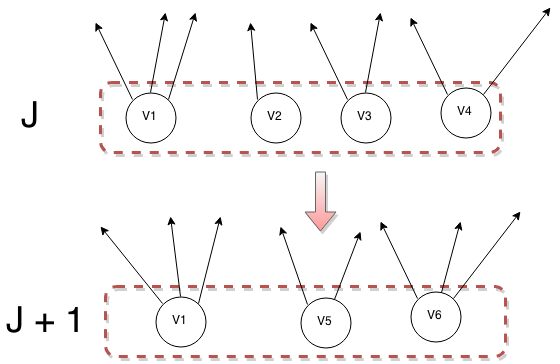
\includegraphics[width=\textwidth]{images/bf_par_3.png}\end{center}}
\end{frame}

\section{Задача many-to-many}


\begin{frame}[fragile]
  \frametitle{Алгоритм Флойда}
  \begin{itemize}
    \item В некоторых случаях классический алгоритм оказывается медленнее наивных алгоритмов
    \item Для каждой вершины можно использовать любой алгоритм поиска кратчайшего пути
  \end{itemize}
\end{frame}


\begin{frame}[fragile]
  \frametitle{Наивная параллельная версия}
\begin{algorithm}[H]
\begin{algorithmic}[1]
\Procedure{AllPairsPar1}{$G$}
\State \textbf{return} {\Call {HandleVertices}{$G, 0, |G.vertices|$}}
\EndProcedure
\State
\Procedure{HandleVertices}{$G, startVertex, endVertex$}

\If {$endVertex - startVertex < threshold$} 
	\State $distances \gets$ run Bellman-Ford for $[startVertex, endVertex)$
	\State \textbf{return} $distances$	
\Else	
	\State $midV \gets (startVertex + endVertex) / 2$ 
	\State \begin{varwidth}[t]{\linewidth}fork2(\par
        \hskip\algorithmicindent {\Call {HandleVertices}{$G, startV, midV$}},\par
        \hskip\algorithmicindent {\Call {HandleVertices}{$G, midV, endV$}});
      \end{varwidth}
	
\EndIf

\EndProcedure
\end{algorithmic}
\end{algorithm}
\end{frame}

\begin{frame}[fragile]
  \frametitle{Алгоритм для объединенного графа}
    {\vspace{-2em}\begin{center}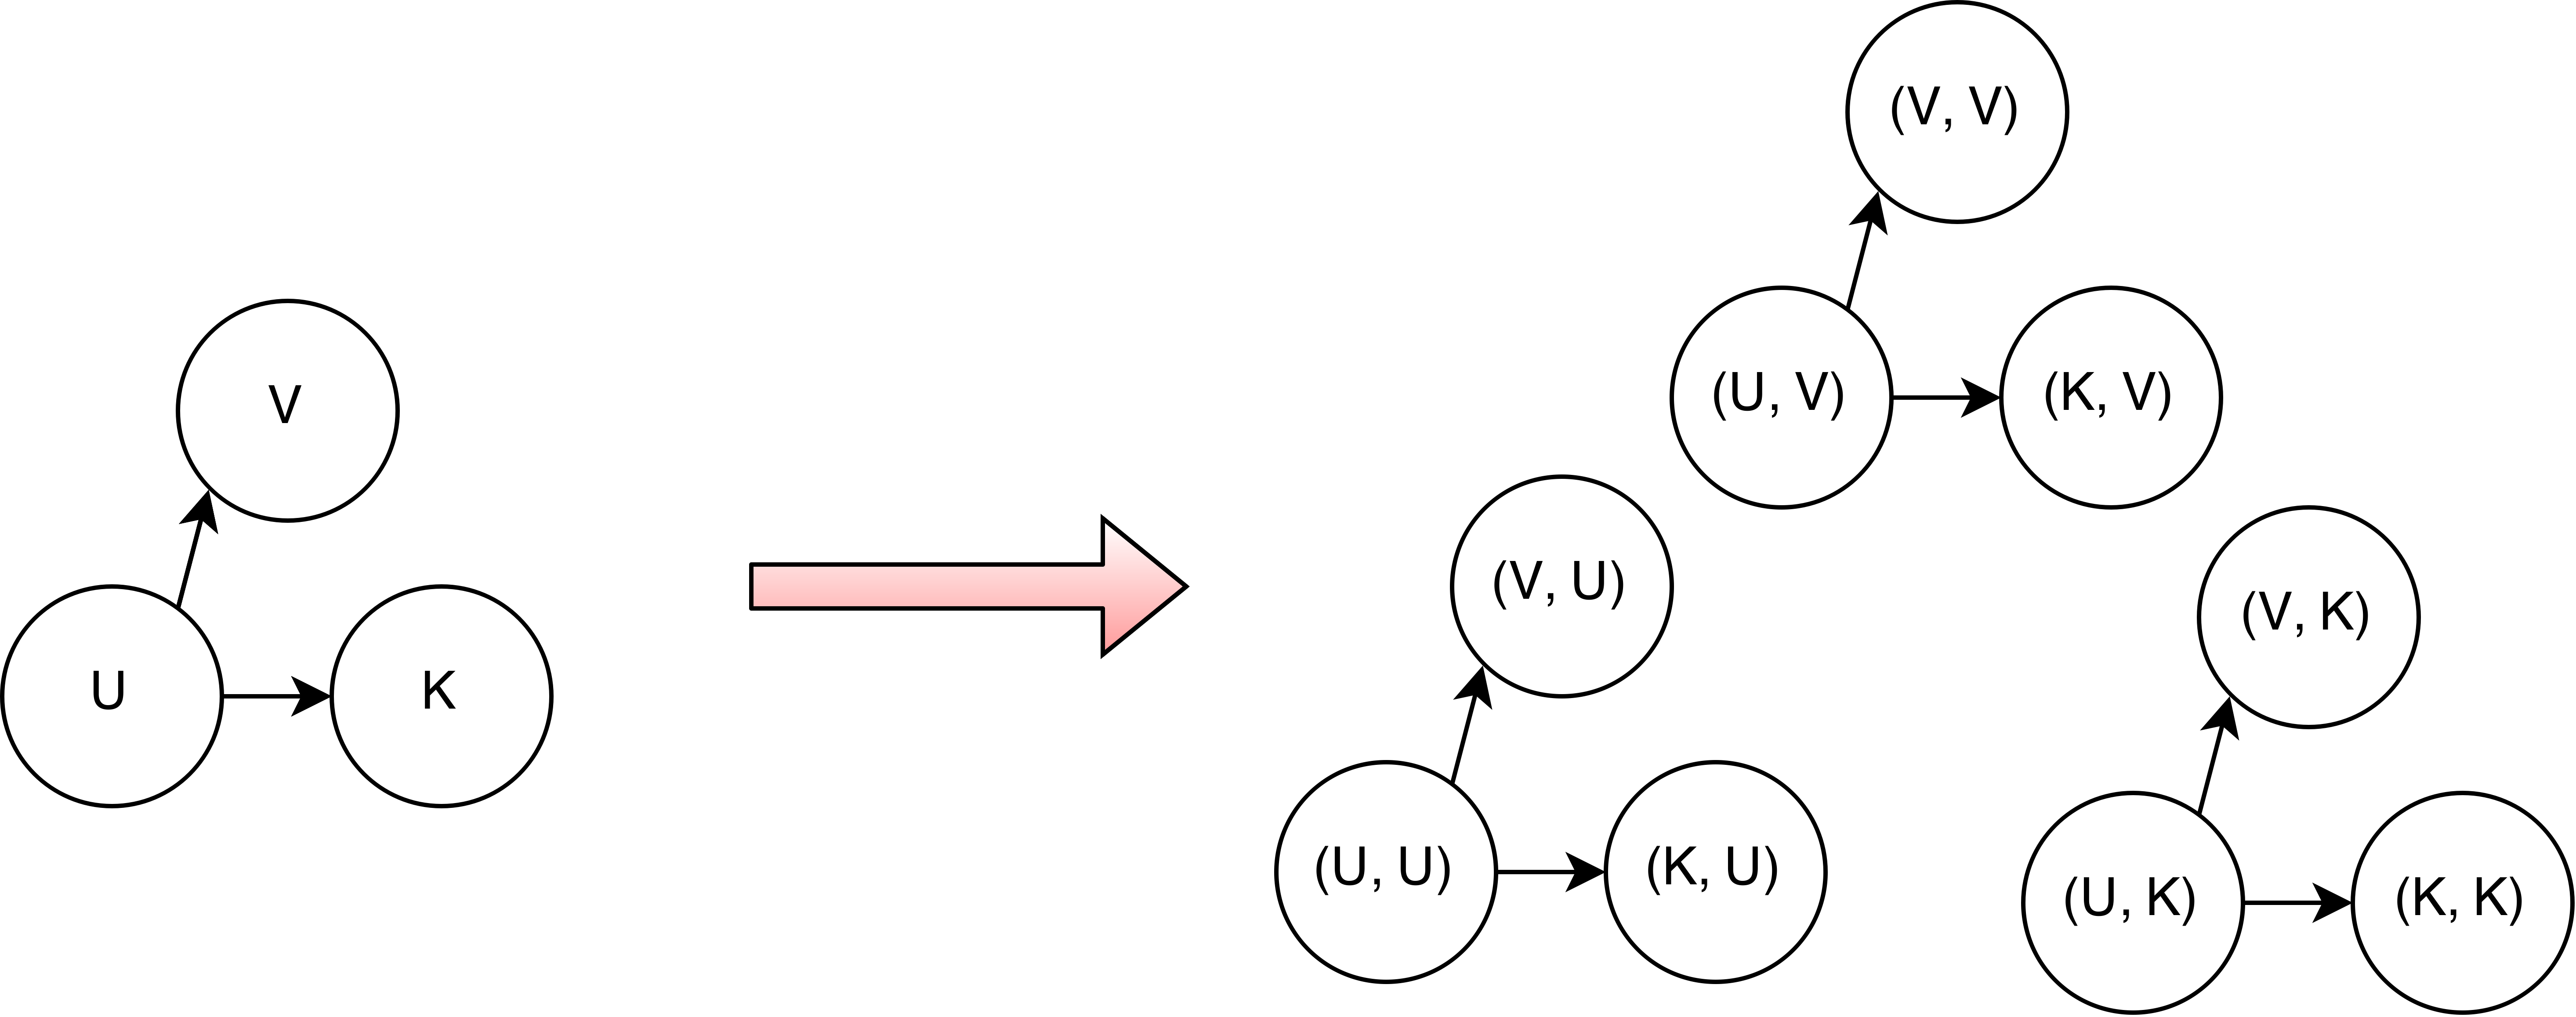
\includegraphics[width=\textwidth]{images/floyd_par_2.png}\end{center}}

\end{frame}

\begin{frame}[fragile]
  \frametitle{Алгоритм для социальных графов}
  \begin{itemize}
    \item Основан на теории "Шести рукопожатий"
    \item Работает не неориентированных невзвешенных социальных графах
    \item Использует идею динамического программирования
  \end{itemize}
\end{frame}

\begin{frame}[fragile]
  \frametitle{Идея}
    {\vspace{-2em}\begin{center}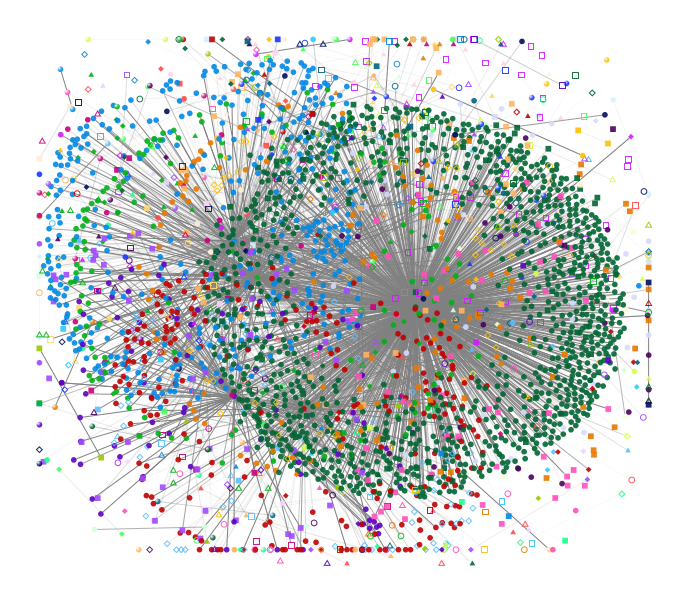
\includegraphics[width=0.8\textwidth,height=0.8\textheight]{images/floyd_social_1.png}\end{center}}

\end{frame}

\begin{frame}[fragile]
  \frametitle{Идея}
    {\vspace{-2em}\begin{center}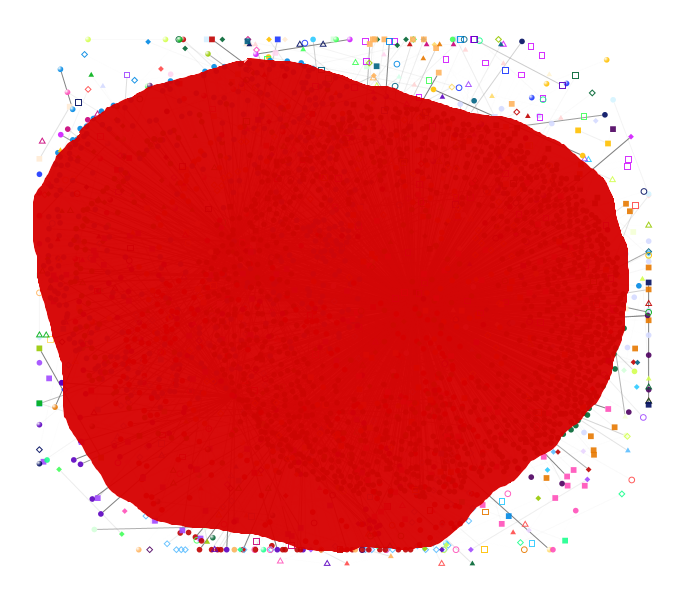
\includegraphics[width=0.8\textwidth,height=0.8\textheight]{images/floyd_social_2.png}\end{center}}

\end{frame}

\begin{frame}[fragile]
  \frametitle{Динамика для большего множества}
    \begin{itemize}
    	\item Посчитаем расстояние от базовой вершины до всех других
    	\item Каждая из вершин $u$ может находится только в $[dist[base][u]-K, dist[base][u]+K]$ слоях
		\item Будем поддерживать две динамики $mask$ и $calc$. Причем $mask[u][i]$ - сабсет вершин, расстояние от которых до $u$ равно $i$. В свою очередь $calc[u][i]$ - не более $i$
	\end{itemize}
\end{frame}

\begin{frame}[fragile]
  \frametitle{Пересчет значении динамики}
\begin{equation}
mask[v][i] = \neg calc[v][i - 1] \wedge \bigvee_{\exists (u, v) \in E} mask[u][i - 1] 
\end{equation}

\begin{equation}
calc[v][i] = calc[v][i - 1] \vee mask[v][i]
\end{equation}

\end{frame}

\begin{frame}[fragile]
  \frametitle{Преимущества подхода}
\begin{itemize}
  \item Пересчет расстояний для группы вершин выполняется быстрее за счет битовых операций.   
  \item Все битовые операции выполняются без выделения дополнительной памяти. 
  \item Нет необходимости в построении следующего фронтира по предыдущему в процессе обработки
  \item Каждый из получившихся фронтиров довольно большой, что увеличивает его способность к 
  \item Все остальные этапы также хорошо параллелятся
\end{itemize}

\end{frame}


\section{Результаты}

\begin{frame}[fragile]
  \frametitle{Сравнение параллельных версий Беллмана-Форда}
\begin{table}
\centering
\begin{tabular}{l|ccc|cc|cc}  
Algo №& \multicolumn{3}{c}{Complete} & \multicolumn{2}{c}{BalancedTree} & \multicolumn{2}{c}{SquareGrid} \\
& TS & + & - & 0.5 & 1 & + & +- \\
\hline\hline
1 & 2.43 & 4.65 & nc & 116.31 & 9.04 & 5.49 & 13.40\\  
2 & 5.17 & 0.18 & 10.84 & 3.59 & 3.08 & 5.92 & 7.10  \\
3 & 44.63 & 0.37 & 23.55 & 0.44 & 0.31 & 4.42 & 0.58 \\
\end{tabular}
\caption{Типичные графы}
\label{graph_description}
\end{table}


\begin{table}
\centering
\begin{tabular}{l|ccc|ccc}  
Algo №& \multicolumn{3}{c}{RandomSparse} & \multicolumn{3}{c}{RandomDense}\\
& 0.5+  & 0.5- & 0.96+ & 0.5+ & 0.5- & 0.96+\\
\hline\hline
1 & nc & nc & 24.35 & nc & nc & 5.01 \\  
2 & 2.77 & 14.68 & 2.42 & 0.48  & 6.38  & 0.46 \\
3 & 0.98 & 22.59 & 0.76  & 0.60  & 10.25 & 0.71 \\
\end{tabular}
\caption{Случайные графы}
\label{graph_description}
\end{table}

\end{frame}


\begin{frame}[fragile]
  \frametitle{Расстояние между каждой парой вершин социального графа}

\begin{table}
\centering

\begin{tabular}{l|c}  
Алгоритм & Twitter graph\\
\hline\hline
Наивная параллельная версия & 427.217 \\  
Алгоритм для социальных графов & 210.322  \\
\hline
\end{tabular}

\caption{Сравнение алгоритмов}
\label {table:algo_floyd_comparison}
\end{table}
  
\end{frame}

\section{Выводы}


\plain{}{Вопросы?}

\end{document}
